
$\mathcal{L}_{\text{Actor}}$, $\mathcal{L}_{\text{Critic}}$, $\mathcal{L}_{\text{Actor-Ind}}$, and $\mathcal{L}_{\text{Critic-Ind}}$ create four interchangeable combinations of learning updates where one or both of the actor and critic loss can be dependent or \textit{indirectly} dependent on the scale of $Q$. We will compare all four update variants, although we are mainly interested in evaluating the two extremes: ``Dep. Actor, Dep. Critic'' ($\mathcal{L}_{\text{Actor}}$, $\mathcal{L}_{\text{Critic}}$) and ``Ind. Actor, Ind. Critic'' ($\mathcal{L}_{\text{Actor-Ind}}$, $\mathcal{L}_{\text{Critic-Ind}}$). Our experimental setup allows for a direct ablation where all other details can be held fixed. Appendix \ref{app:implementation} includes additional implementation details. Our experiments focus on three main questions: \textbf{1)} Do scale-resistant actor-critic objectives offer empirical benefits in challenging generalization problems? \textbf{2)} If so, can these gains be attributed to multi-task return scaling? and \textbf{3)} What new applications of memory-based policies might be unlocked by improvements in multi-task optimization without task labels?

\begin{figure}[h!]
    \centering
    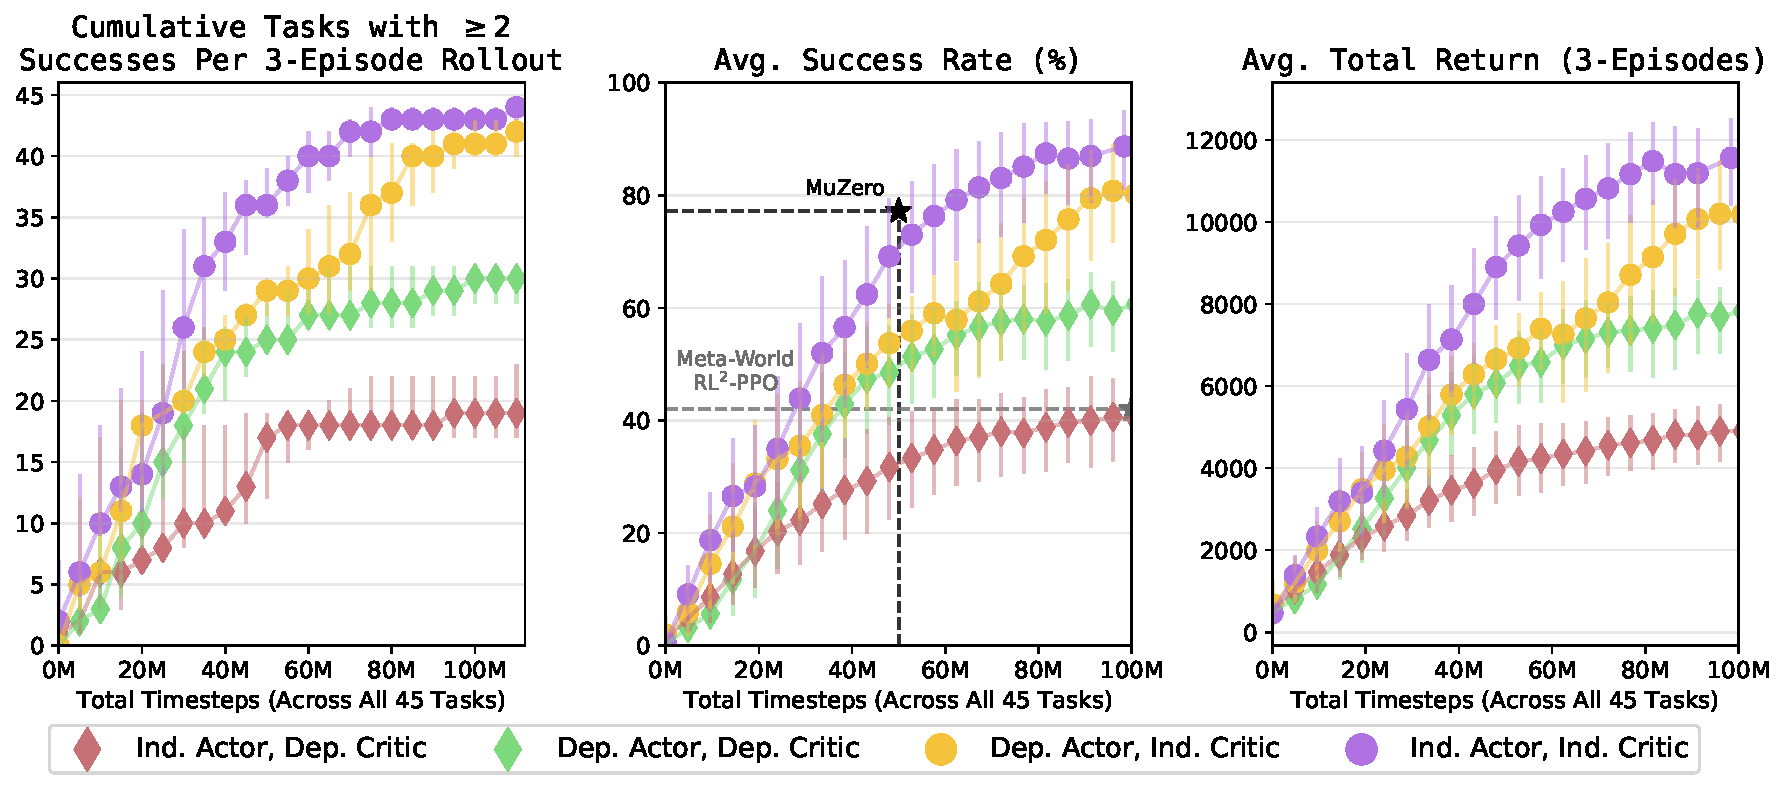
\includegraphics[width=\textwidth]{figures/final/metaworld_main_text-2.pdf}
    \caption{\textbf{Meta-World ML45 Train Task Results.} \textbf{(Left)} Coverage of the $45$ manipulation skills measured by an adaptation horizon success rate $\geq 2/3$. \textbf{(Center)} Average success rate over tasks, variants, and $3$-episode rollouts. Reference scores for MuZero and RL$^2$-PPO are gathered from results in \cite{yu2020meta, anand2022procedural}. \textbf{(Right)} Total return over a $3$-episode adaptation horizon, averaged across tasks and variants. All error bars indicate the maximum and minimum metric across three random trials.}
    \label{fig:metaworld_results}
    \vspace{-4mm}
\end{figure}

\paragraph{Meta-World ML45.} ML45 is a challenging suite of $45$ robotic manipulation meta-RL tasks. We argue that much of ML45's difficulty can be attributed to variance in return scales: ML45's training tasks are designed to have similar optimal returns, but they have different levels of difficulty, which causes the scale of $Q$-values to diverge early in training. The PopArt method of normalizing $Q$ per task may help balance optimization. Methods built on the original Meta-World results normalize the returns of each task separately \cite{garage}, which is a simpler approach to the same idea. We force all task identification to be learned within the context of our memory policy so that one-hot labels and the total task size ($45$) do not influence training. The training environment samples a new task between meta-rollouts and the task identity is not included in the observation. Every task shares a single critic head, and all experience is added to a shared replay buffer sampled uniformly at random. 

Figure \ref{fig:metaworld_results} compares the four combinations of learning updates described in Section \ref{sec:method}. Actor and critic loss terms that do not scale directly with the $Q$-values of each task improve skill coverage, overall success rate, and cumulative return across $3$-episode adaptation horizons. Replacing $Q$ regression with two-hot classification appears to be the most important change, although substituting the weighted IL policy update improves performance and sample efficiency. Full learning curves for all $45$ tasks are plotted in Appendix \ref{app:results} and highlight the uneven learning progress (and therefore $Q$-value scale) of tasks throughout training. With a sample budget of $100$M timesteps, our off-policy Transformers trained by max likelihood losses $(\mathcal{L}_{\text{Actor-Ind}}, \mathcal{L}_{\text{Critic-Ind}})$ more than double the success rate of Meta-World's original RL$^2$ result over the same sample limit while maintaining a $1.4\times$ improvement on its performance at $400$M timesteps. Our simple one-step $Q$-learning matches more complex value updates like MuZero \cite{schrittwieser2020mastering} at its reported $50$M timestep budget \cite{anand2022procedural}. We use a general Transformer architecture that would be equally applicable to any sequence modeling problem, but our results are also comparable to recent work such as HTrMRL \cite{shala2024hierarchical} (success rate $\approx 85
\%$) that use architectures specialized for multi-episodic RL. 

\begin{wrapfigure}{r}{.49\textwidth}
\vspace{-15mm}
\begin{center}
    \centering
    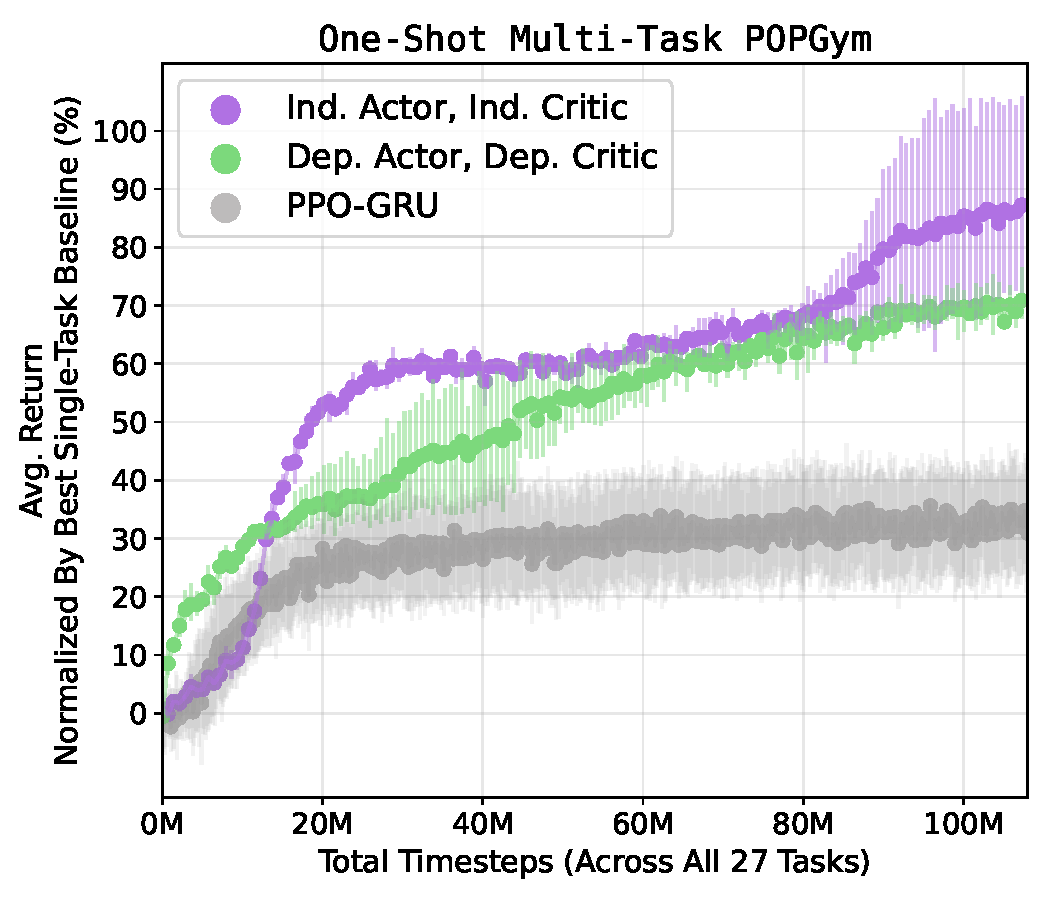
\includegraphics[width=.48\textwidth]{figures/final/popgym_results_summary_final.pdf}
    \vspace{-2mm}
    \caption{\textbf{Multi-Task POPGym Results.} Returns are normalized by single-task experts trained for $15$M timesteps. Error bars indicate the maximum and minimum returns across three trials.}
    \label{fig:popgym_results}
\end{center}
\vspace{-3mm}
\end{wrapfigure}
\paragraph{Multi-Task POPGym.} Meta-World is designed as a meta-learning benchmark, but its adaptation does not require long-term memory. POPGym \cite{morad2023popgym} is a suite of zero-shot POMDP problems. Many POPGym tasks are explicit tests of long-term recall, but others involve state and variant estimation from previous actions and rewards. We use a simple observation and action space padding approach to create a multi-task version of POPGym: we combine all $27$ tasks where both the action space and observation space have dimension $< 30$. It is not clear whether zero-shot performance in this setting can be compared against single-task POPGym results, as a strong agent may need to lose valuable time identifying which of the $27$ memory games it is currently playing. Therefore, we evaluate in a one-shot setting where the first trial is a free exploration window used to determine which task is active so that the second trial creates a fair comparison to single-task results \cite{stadie2018some}. Importantly, we avoid ``spoiling'' any memory challenges for the second trial by randomly resetting to a new variant of the same task.

We compare Transformers trained by the ``indirect'' and $Q$-dependent update against the on-policy PPO agent from the POPGym codebase \cite{morad2023popgym} using the best sequence model from the original benchmark (a GRU RNN \cite{cho2014learning}). Figure \ref{fig:popgym_results} aggregates the results across all $27$ tasks with returns scaled between a random policy and the best single-task result (of any sequence model) that appears in \citet{morad2024reinforcement}. Single-task reference scores are given a budget of $15$M timesteps, while our multi-task agents see a total of $100$M across all $27$ tasks and train on reward signals for approximately half of those timesteps. Both Transformer learning updates outperform PPO-GRU but are relatively comparable to each other. This may not be surprising because POPGym tasks have similar learning curves and returns bounded in $[-1, 1]$. However, many of these tasks have sharp short-term credit assignment where the advantage surface of an accurate value function would be steep. We expect the standard $\mathcal{L}_{\text{Actor}}$ update to be a significant improvement in online exploration, so it is encouraging that the offline-style $\mathcal{L}_{\text{Actor-Ind}}$ can exceed its performance after $15$M total timesteps. Learning curves for each task can be found in Appendix \ref{app:results}.


\begin{figure}[h!]
    \vspace{-2mm}
    \centering
    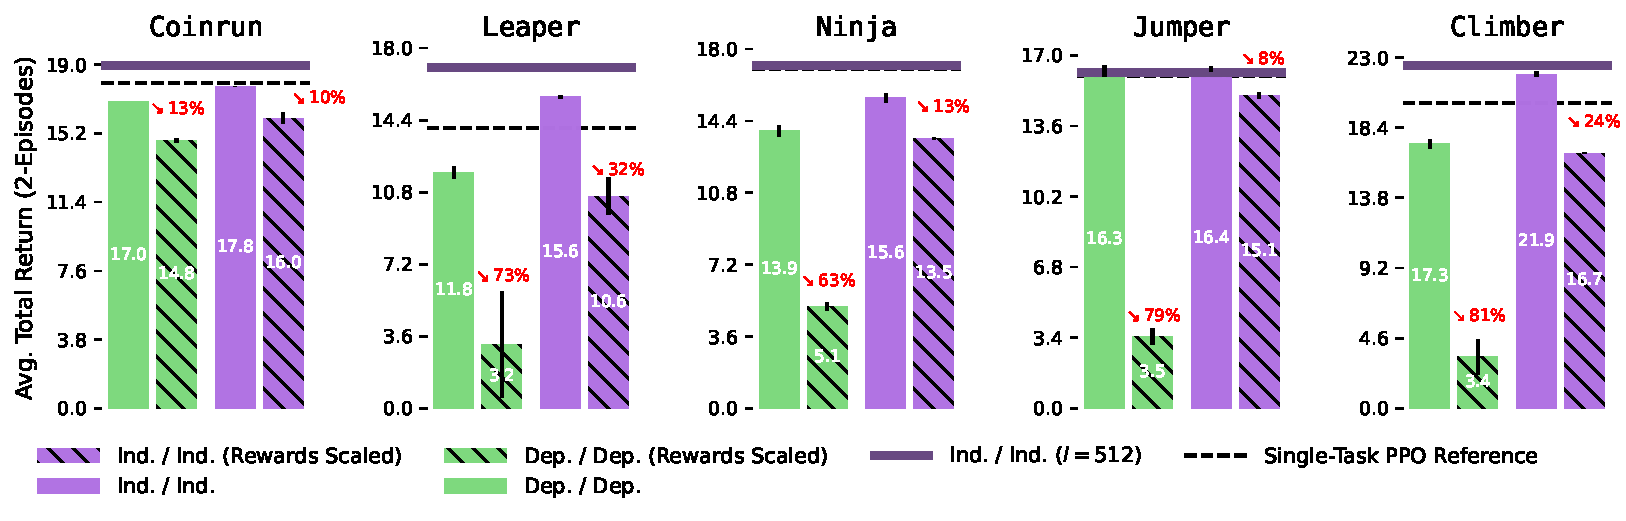
\includegraphics[width=.9\textwidth]{figures/final/procgen_reward_scaling_summary.pdf}
    \vspace{-3mm}
    \caption{\textbf{Return Scales in Multi-Game Procgen.} We evaluate over $2$ episodes in unseen levels after optimizing default or rescaled reward functions. Scores are averaged over two model checkpoints and converted to the default scale. Error bars indicate the difference between two $275$M timestep trials.}
    \vspace{-2mm}
    \label{fig:popgym_easy_mode}
\end{figure}


\paragraph{Multi-Game Procgen.} Procgen \cite{cobbe2020leveraging} creates $16$ video games with an infinite variety of procedurally generated levels. If memory-based actor-critic learning is bottlenecked by the scale of returns across multiple tasks, we should be able to decrease performance by simply rescaling rewards. We begin by training multi-task agents across $2$k levels of five games in easy mode. Solid bars in Figure \ref{fig:popgym_easy_mode} show the performance on unseen test levels, where the scale-resistant update offers a slight improvement. 


\begin{figure}[h!]
    \vspace{-3mm}
    \centering
    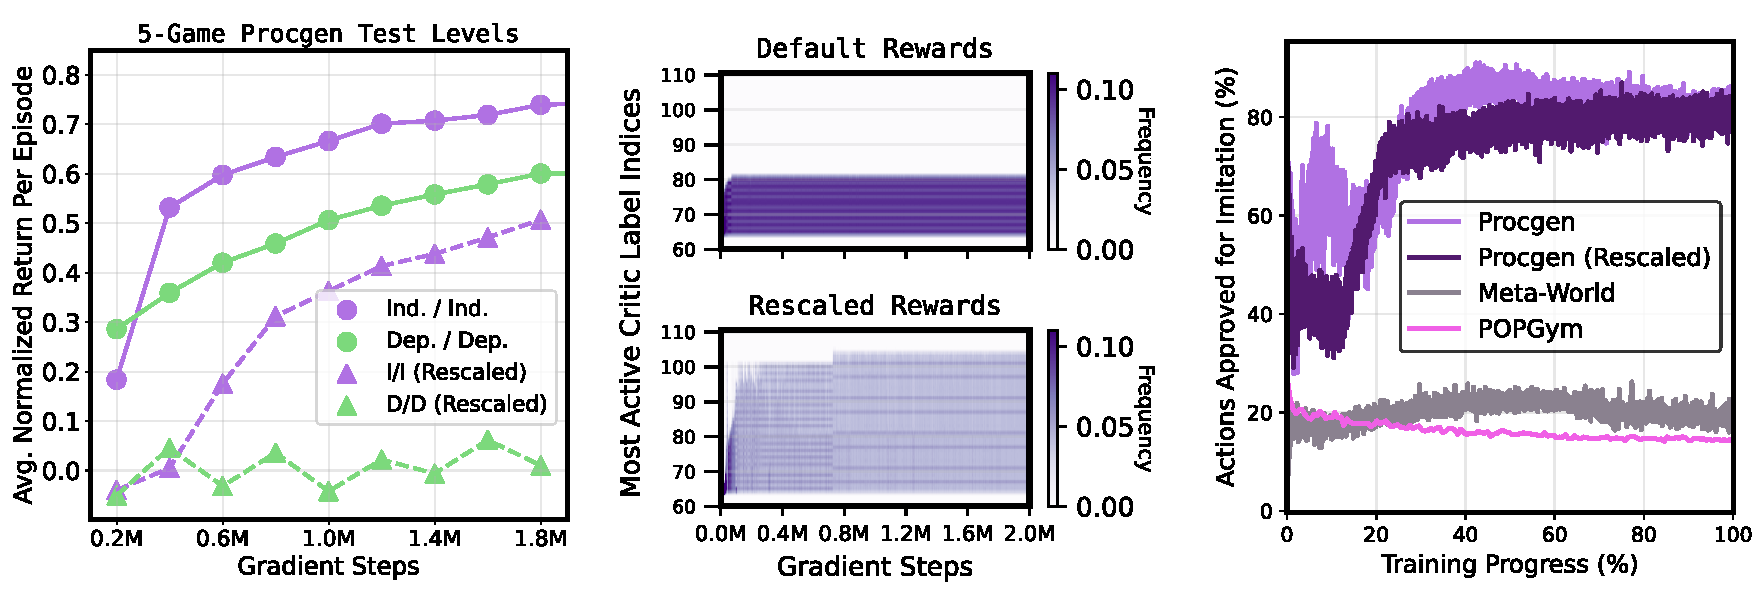
\includegraphics[width=\textwidth]{figures/final/procgen_combined.pdf}
    \caption{\textbf{Learning from Rescaled Returns.} \textbf{(Left)} Procgen test level returns normalized across games according to the standard benchmark scale \cite{cobbe2020leveraging}. \textbf{(Center)} Frequencies of the critic classification label index with the highest probability throughout training. We trim the y-axis to the portion of \texttt{symlog} \cite{hafner2023mastering} space that is relevant to Procgen. \textbf{(Right)} The value of $\mathcal{L}_{\text{Actor-Ind}}$ binary advantage weights create an estimate of the percentage of the replay buffer currently being imitated.}
    \label{fig:procgen_analysis}
\end{figure}


Our multi-task Procgen environment randomly selects a new game between resets, which does not account for how episode lengths depend on the agent's skill (Figure \ref{fig:procgen_frame_counts}). We retrain new policies from scratch but scale the rewards of the easiest task (Coinrun) by $\times 100$ while dividing the rewards of the task the agent spends the most timesteps interacting with (Climber) by $10$. We would expect the scale of $\mathcal{L}_{\text{Actor}}$ and $\mathcal{L}_{\text{Critic}}$ to be dominated by Coinrun so that optimization variance overshadows the objectives of the other environments even after learning in Coinrun converges. Hatched bars in Figure \ref{fig:popgym_easy_mode} show this is indeed the case, with methods recovering most of their original performance in Coinrun while failing to improve in the other four games. The ``Ind. / Ind.'' update is far less impacted by the new return scales even though they decrease efficiency in terms of gradient steps (Figure \ref{fig:procgen_analysis} Left). Fig. \ref{fig:procgen_analysis} (Center) reveals a simple explanation where the broader range of returns approximately doubles the number of frequently used labels our critics need to learn to classify. Multi-task Transformer policies are commonly trained by imitation learning, and Fig. \ref{fig:procgen_analysis} (Right) highlights why $\mathcal{L}_{\text{Actor-Ind}}$ is so effective for training multi-task Transformer policies with online RL: the policy update reduces to IL on a dynamic percentage of the replay buffer, but the ability to ignore a fraction of the dataset automatically allows for self-improvement in a way that standard IL does not.

\begin{figure}[h!]
    \vspace{-1mm}
    \centering
    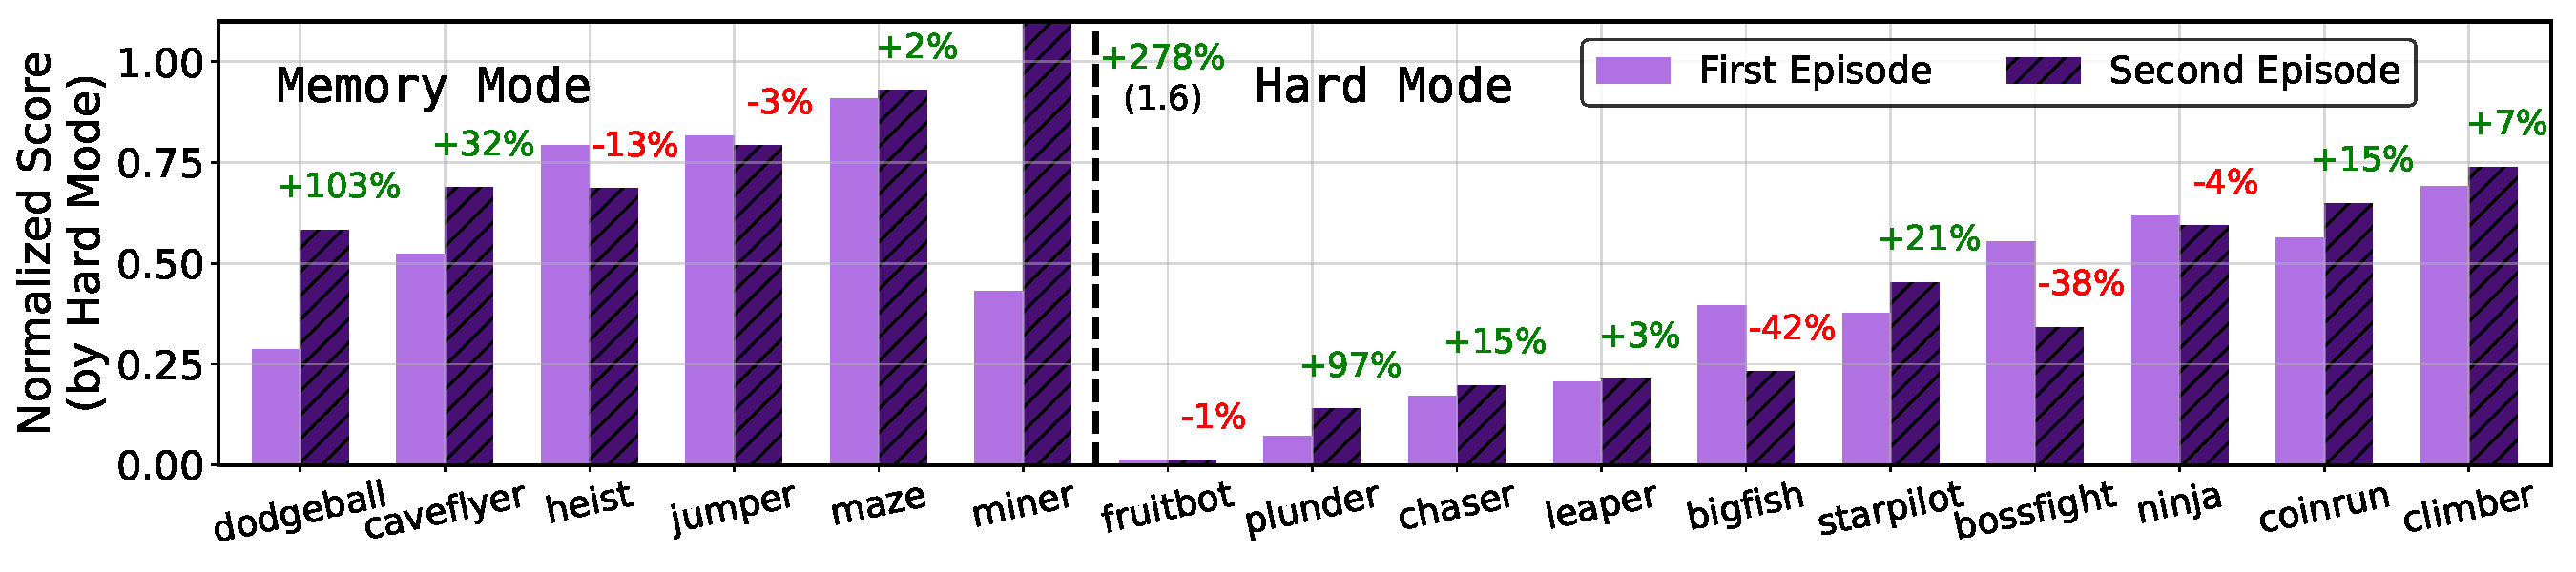
\includegraphics[width=.9\textwidth]{figures/final/procgen_memory_hard_new6.pdf}
    \vspace{-4mm}
    \caption{\textbf{Multi-Task Procgen in Memory-Hard Mode.} We measure policy performance across the two episodes of its adaptation window. Results are averaged over $30$M  frames in unseen test levels. }
    \label{fig:procgen_memory}
    \vspace{-1mm}
\end{figure}

Inspired by the success of the ``Ind. / Ind.'' learning update in the easy distribution of $5$ games, we train a larger $24$M parameter Transformer with a context length of $l=768$ frames on all $16$ Procgen games simultaneously. We default to the standard ``hard'' level distribution but increase the difficulty to the (rarely attempted) ``memory'' mode in the $6$ games it is available. Results after $2.7$B frames are highlighted in Figure \ref{fig:procgen_memory}. The agent does improve its performance on the second attempt of unseen levels --- particularly in memory games where partial observability makes adaptation most useful.

\begin{figure}[h!]
    \vspace{-2mm}
    \centering
    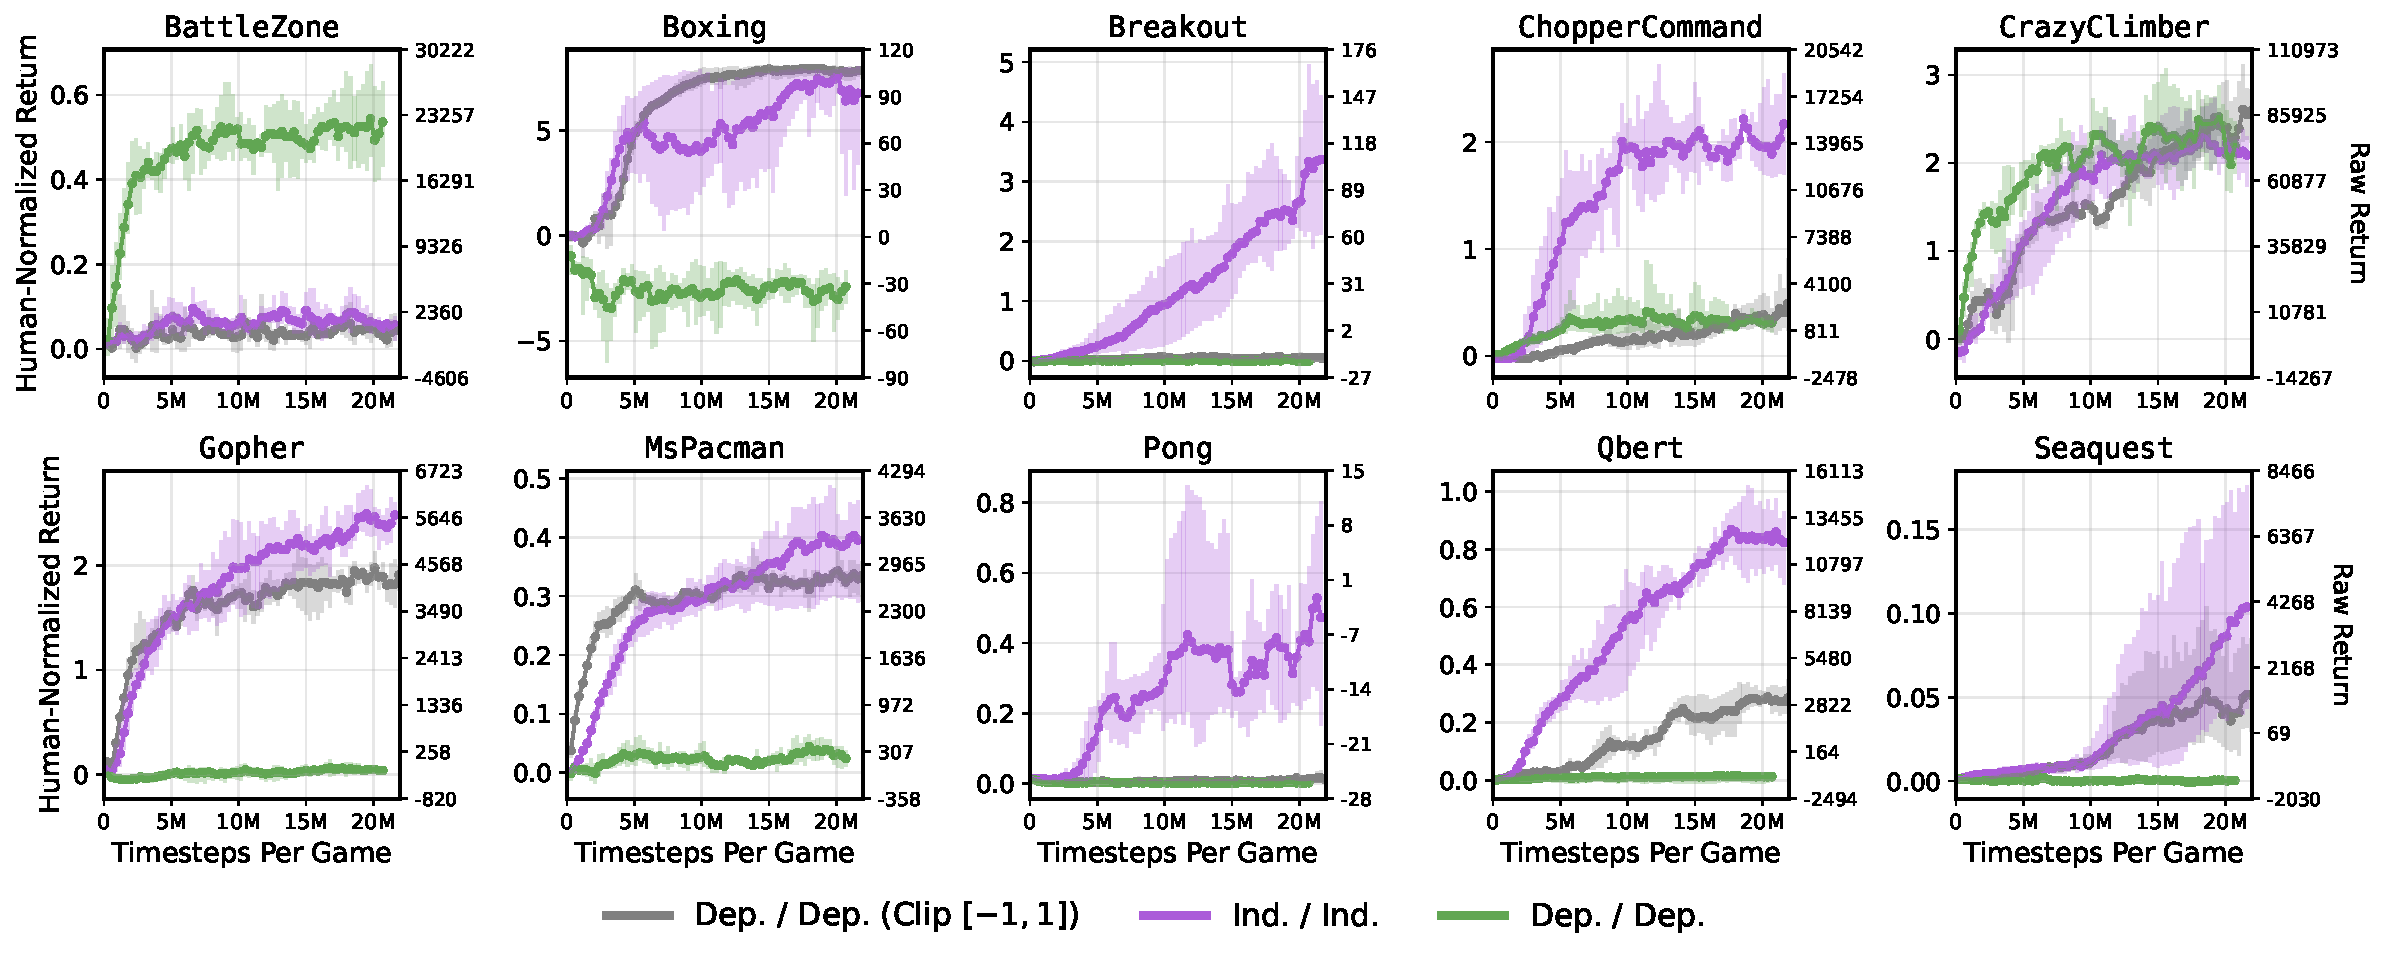
\includegraphics[width=.98\linewidth]{figures/final/atari_results_larger_font.pdf}
    \vspace{-2mm}
    \caption{\textbf{Multi-Game Atari Without Reward Clipping.} We train a single policy on $10$ games simultaneously. Results are plotted relative to human performance (left axis) and the raw scale of returns (right axis). Error bars denote the maximum and minimum over four random trials.}
    \label{fig:atari_result}
    \vspace{-3mm}
\end{figure}

\paragraph{Multi-Game Atari.} If RL generalization problems lie on axes between meta-RL and MTRL (Section \ref{sec:background}), the ALE \cite{bellemare2013arcade} would represent the multi-task extreme. Super-human performance on Atari does not require adaptation or memory but leads to per-game returns separated by orders of magnitude \cite{hessel2018rainbow}, which motivates the infamous trick of clipping rewards in $[-1, 1]$ \cite{mnih2015human}; clipping stabilizes learning but misaligns agents' training objective from the raw game score used for evaluation. PopArt \cite{hessel2019multi} showed that multi-task training on unclipped rewards is possible when we split critic networks into game-specific output heads with independently normalized targets. Figure \ref{fig:atari_result} revisits this experiment on a smaller scale. However, rather than normalizing a multi-task architecture, we train a single critic on $10$ games with unclipped rewards and let our shared Transformer recover state and task labels implicitly from context sequences (of RGB images). In other words, we are treating the widely studied MTRL Atari setting as a special case of meta-learning in order to isolate the challenge of optimizing returns on different scales. Results are shown in Figure \ref{fig:atari_result}. The scale-resistant update leads to dramatic improvements in $8/10$ games; the default $Q$-dependent update performs best in the two games where returns at random initialization are significant outliers. The standard approach of clipping rewards in $[-1, 1]$ (grey) helps mask the multi-task optimization challenge created by scale-dependent learning updates.

\paragraph{BabyAI.} BabyAI is a suite of partially observed gridworld tasks with simple language instructions \cite{chevalier-boisvert2018babyai}. We create a hybrid multi-task meta-RL problem with the potential for task generalization by randomly generating a train/test split over $68$ of BabyAI's task configurations as provided by the Minigrid simulator \cite{MinigridMiniworld23}. Our agents observe a text description of the their task and have two attempts to adapt to a procedurally generated level layout. Learning curves for all $68$ tasks are provided in Appendix \ref{app:results}. Figure \ref{fig:babyai_main} summarizes our results in the BabyAI domain and reveals another case where scale-independent updates outperform scalar regression. Figure \ref{fig:babyai_icrl} evaluates BabyAI as a multi-episodic adaptation problem by comparing the returns of the first and second attempt in a new level layout. Despite BabyAI's partial observabilty, only a small set of tasks benefit from in-context adaptation over a context length $l=512$. Transformers are clearly capable of learning effective recall over sequences of this length via RL \cite{ni2023transformers, grigsby2024amago}, and we have demonstrated that scale-invariant updates can unlock significant improvement in terms of multi-task training. Therefore we argue that the next step is to train this agent in a domain with sufficient task diversity to evaluate meta-learning over $k > 2$ episodes. XLand Minigrid \cite{nikulin2023xland} is a concurrent effort to augment gridworlds with millions of unique tasks and may be a promising domain for future study.



\begin{figure}[h!]
    \vspace{-2mm}
    \centering
    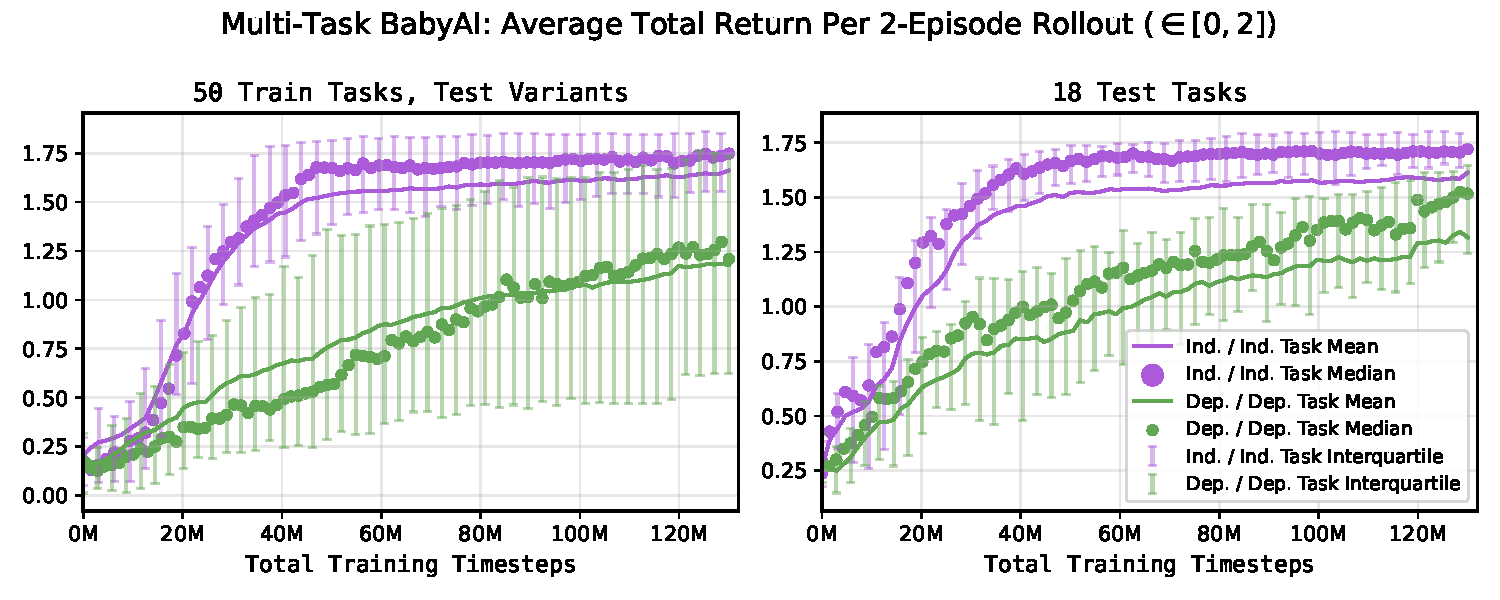
\includegraphics[width=.85\linewidth]{figures/final/babyai_draft_figure_v2.pdf}
    \vspace{-4mm}
    \caption{\textbf{Multli-Task BabyAI.} Results are the average over four training seeds and plotted according to the median, mean, and interquartile range over the task set.}
    \label{fig:babyai_main}
    \vspace{-2mm}
\end{figure}
 
\begin{figure}[h!]
    \vspace{-3mm}
    \centering
    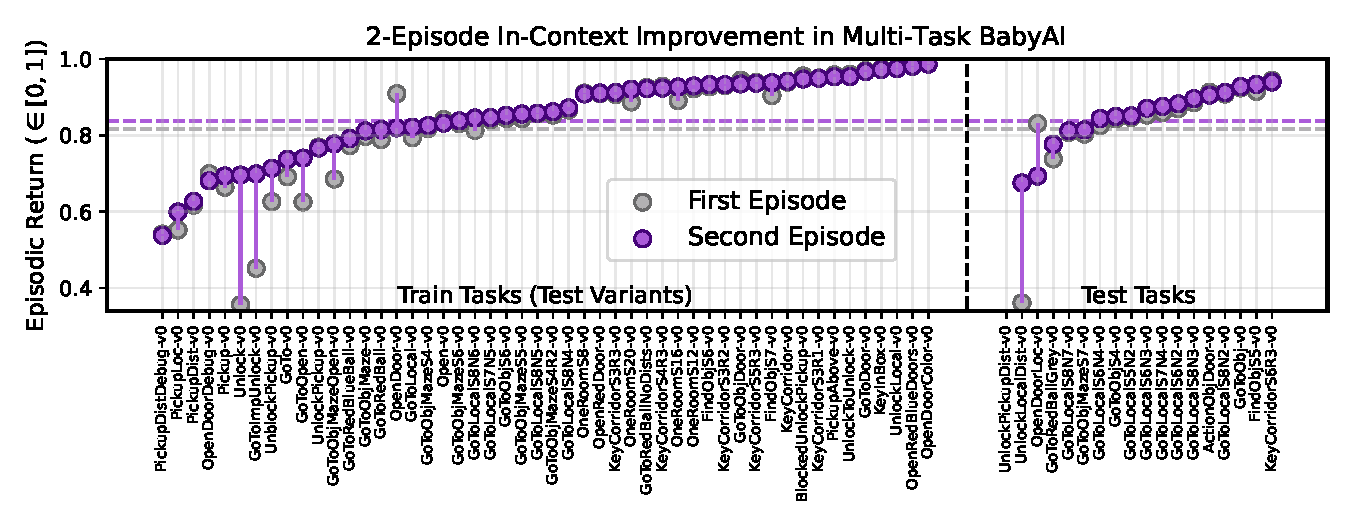
\includegraphics[width=.92\linewidth]{figures/final/icrl_babyai_figure.pdf}
    \vspace{-4mm}
    \caption{\textbf{In-Context BabyAI.} We measure the average return of ``Ind. / Ind.'' agents by attempt in unseen tasks and/or layouts (variants). Results are arbitrarily sorted in order of increasing second-episode return and are the average of four training seeds and $10$M evaluation timesteps.}
    \label{fig:babyai_icrl}
    \vspace{-6mm}
\end{figure}